\chapter{Conductance in the Kondo Regime}\label{cha:kondo_conductance}


    This chapter provides the theoretical and methodological context for the research in this thesis. 
    It begins with an overview  

\begin{figure}[ht]
  \begin{center}
%% includegraphics: comment the following if not using the graphicx package
    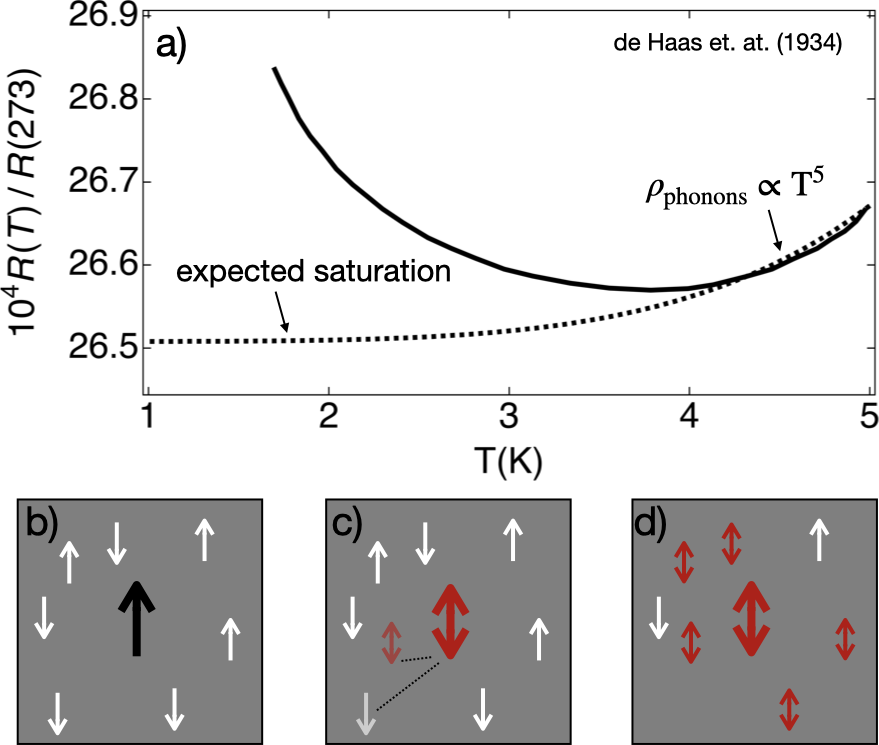
\includegraphics[width=1.0\textwidth]{figures/ch2/crop_PosterFiguresMaster.006.png}
    \caption[Kondo effect in bulk materials]{\label{fig:ch2/kondo_bulkmetal} 
    % For some options that work with pdf\LaTeX, please see this discussion:
    %   \url{http://tex.stackexchange.com/questions/11839}.  
    (\textbf{a}) Temperature dependence of the resistivity, $\rho$. Due to electron-phonon scattering, the resistivity decreases as $T^5$. Due to the Kondo effect, the resistivity will reach a minima before it starts increasing logarithmically with decreasing $\mathrm{T}$. The data used for this figure has been obtained from XXX. (\textbf{b}) A single magnetic impurity (black arrow) is surrounded by conduction electrons (white arrow). (\textbf{c}) Conduction electrons scatter off the localised state resulting in a possible spin flip of both particles, leaving the particles entangled. (\textbf{d}) Continued scattering events build a macroscopic coherent state known as a "Kondo singlet" .
      }
  \end{center}
\end{figure}


\begin{figure}[ht]
  \begin{center}
%% includegraphics: comment the following if not using the graphicx package
    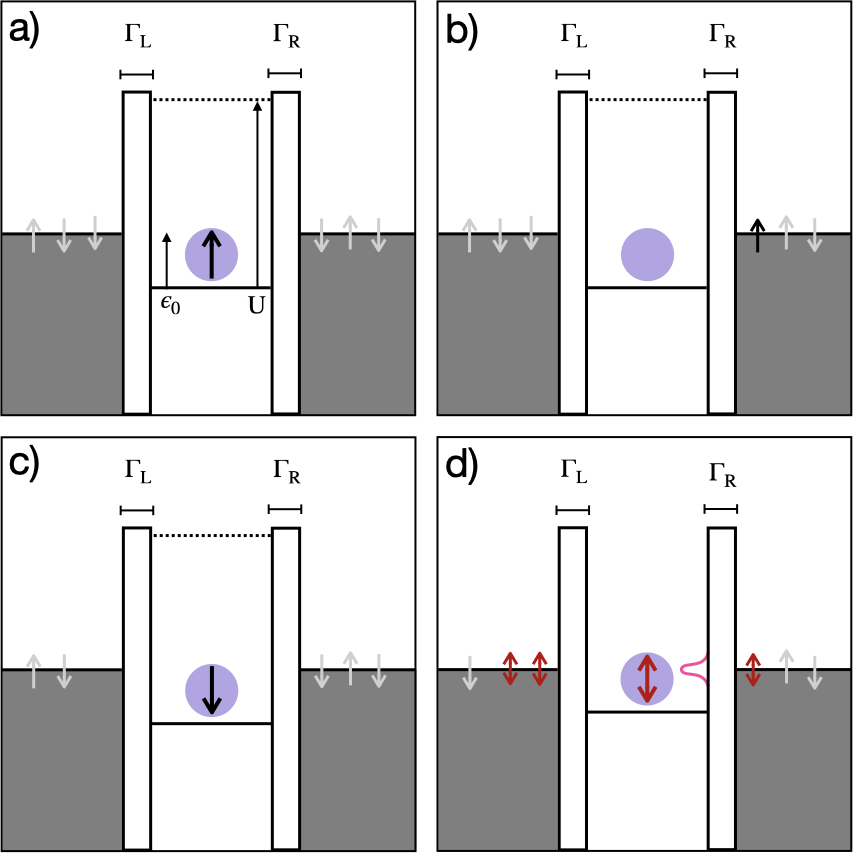
\includegraphics[width=0.8\textwidth]{figures/ch2/crop_PosterFiguresMaster.007.png}
    \caption[Kondo effect in a quantum dot: Coulomb blockade energy diagrams]{\label{fig:ch2/kondo_dot_diagram} 
    % For some options that work with pdf\LaTeX, please see this discussion:
    %   \url{http://tex.stackexchange.com/questions/11839}.  
    A Coulomb blockade energy diagram picture of a Kondo singlet formation in a quantum dot, where the dot acts as the localised spin. The dark grey represents the continuous energy level of electrons in the leads. The white rectangles represent tunnel barriers between the quantum dot and leads. The rate of tunneling is described by the parameter $\Gamma$, the wider (narrower) the barrier, the smaller (larger) the rate of tunneling. (\textbf{a}) The quantum dot has a one spin-degenerate energy level $\mathrm{\epsilon_0}$ occupied by a single electron. The next energy level is separated by the charging energy, $\mathrm{U}$. From Figure~\ref{fig:ch1/dot_intro} we expect zero conductance through the quantum dot. (\textbf{b},\textbf{c}) depict a possible virtual tunneling event where the spin-up electron tunnels out of the dot and a spin-down electron tunnels into the dot within a short time. (\textbf{d}) These virtual tunnel events involving spin-flips lead to a correlated state, the Kondo singlet. This state can be pictured as a narrow density of states formed at the Fermi energy of the leads. If a Kondo singlet has been formed, we will measure enhanced conductance though the quantum dot even as the energy level of the dot is below the energy level of the leads. NOTE: The formation of the Kondo singlet requires an odd number of electrons in the quantum dot.
      }
  \end{center}
\end{figure}


\begin{figure}[ht]
  \begin{center}
%% includegraphics: comment the following if not using the graphicx package
    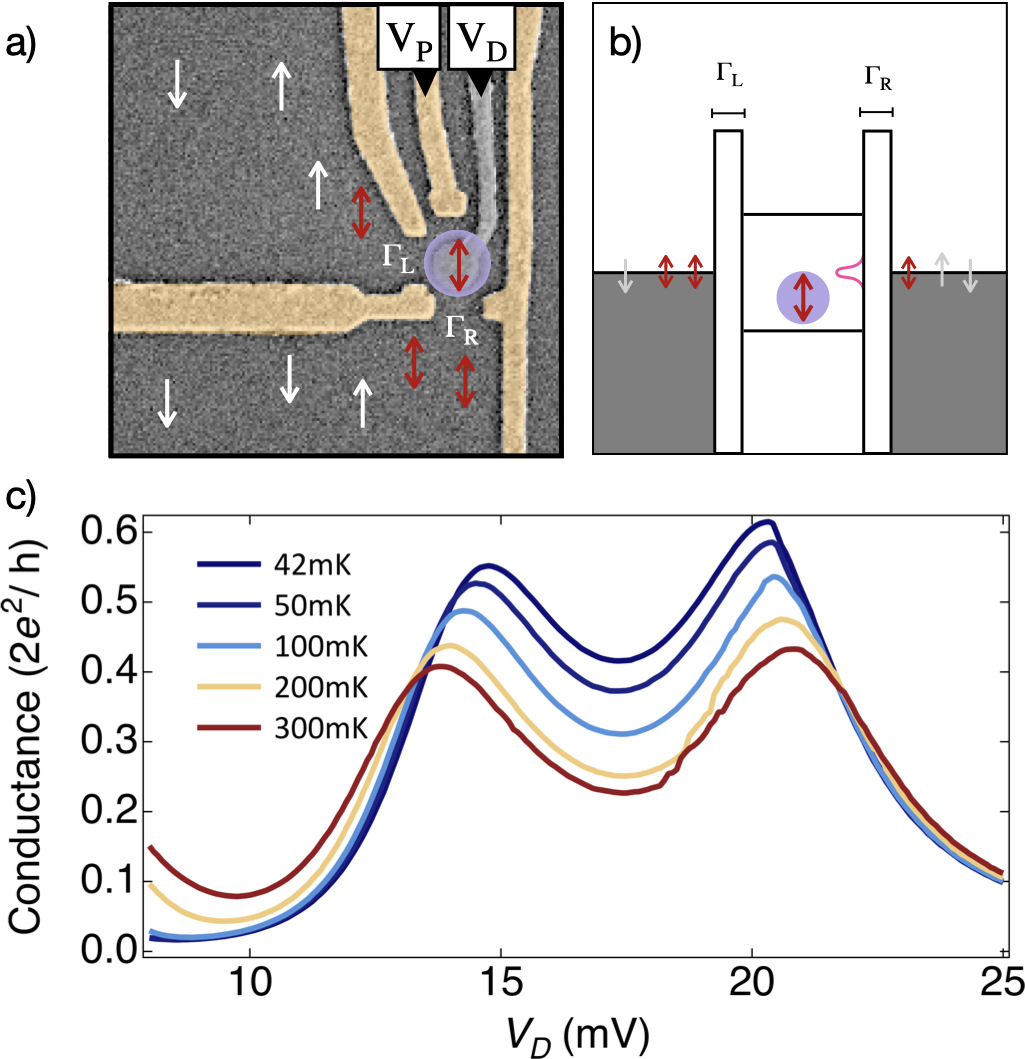
\includegraphics[width=0.8\textwidth]{figures/ch2/crop_PosterFiguresMaster.008.png}
    \caption[Kondo effect in a quantum dot in the Kondo regime]{\label{fig:ch2/kondo_regime_conductance} 
    % For some options that work with pdf\LaTeX, please see this discussion:
    %   \url{http://tex.stackexchange.com/questions/11839}.  
    (\textbf{a}) An SEM image of the gates used to define a quantum dot. The dot contains an odd number of electrons and the tunnel barriers are tuned so that a Kondo singlet is formed. (\textbf{b}) A Coulomb blockade energy diagram picture of a Kondo singlet. As the dot energy falls below the energy level of the leads there is enhanced conductance due to virtual tunneling events through the quantum dot. (\textbf{c}) Data showing the temperature dependence of conductance through a quantum dot with a Kondo singlet formed. In the even occupied sides conductance decreases as the temperature is lowered. On odd occupation a Kondo singlet forms and conductance increases with decreasing temperature.}
  \end{center}
\end{figure}